\section{VECTƠ TRONG MẶT PHẲNG TỌA ĐỘ}
\subsection{TÓM TẮT LÝ THUYẾT}

\subsubsection{Trục tọa độ}
\vspace{-0.6cm}

\immini{
	\begin{itemize}	
	\item [\iconMT] Trục tọa độ là đường thẳng trên đó xác định một điểm gốc là $O$ và một vec tơ đơn vị $\overrightarrow{e}$, kí hiệu $(O,\overrightarrow{e})$.
	\item [\iconMT] Xét điểm $M$ trên trục $(O,\overrightarrow{e})$, ta luôn có $\overrightarrow{OM}=k\overrightarrow{e}$. Khi đó $k$ là tọa độ của $M$ trên trục đã cho.
	\end{itemize}
}{
\begin{tikzpicture}[scale=1, line join=round, line cap=round,>=stealth]
	\draw[->] (-1,0)--(4,0) node [below]{$x$};
	\draw[->,thick] (0,0)--(1,0) node [below]{$\overrightarrow{e}$};
	\draw (0,0) node[above left]{$O$};
	\tkzDefPoints{0/0/O,3/0/M}
	\tkzDrawPoints[size=2,fill=black](O,M)
	\tkzDrawSegments(O,M)
	\tkzLabelPoints[above](M)
\end{tikzpicture}}

\vspace{-0.6cm}
\subsubsection{Hệ trục tọa độ}
\vspace{-0.6cm}

\immini{Hệ trục tọa độ bao gồm 2 trục vuông góc nhau (hình vẽ), kí hiệu $(O,\overrightarrow{i},\overrightarrow{j})$ hay $Oxy$.
		\begin{tcolorbox}[colframe=orange,colback=white,boxrule=0.2mm]
				\begin{itemize}
					\item  $O$ là gốc tọa độ; $Ox$ là trục hoành; $Oy$ là trục tung;
					\item $\overrightarrow{i}$, $\overrightarrow{j}$ là các vec tơ đơn vị và $|\overrightarrow{i}|=|\overrightarrow{j}|=1$.
				\end{itemize}
			\end{tcolorbox}
}{\begin{tikzpicture}[smooth,font=\footnotesize,scale=0.8,>=stealth]
		\draw[->] (-1,0)--(4,0) node [below]{$x$};
		\draw[->] (0,-1)--(0,3) node [left]{$y$};
		\draw[->,thick] (0,0)--(1,0) node [below]{$\overrightarrow{i}$};
		\draw[->,thick] (0,0)--(0,1) node [left]{$\overrightarrow{j}$};
		\draw (0,0) node[above left]{$O$};
	\end{tikzpicture}
}

\vspace{-0.6cm}
\subsubsection{Tọa độ của vectơ}
\vspace{-0.6cm}

\immini{\begin{itemize}	
	\item [\iconMT] \indam{Định nghĩa:} Với mỗi vectơ $\vec{u}$ trên mặt phẳng $Oxy$, có duy nhất cặp số $(x_0;y_0)$ sao cho $\vec{u}=x_0\vec{i}+y_0\vec{j}$. Ta nói $\vec{u}$ có tọa độ là $(x_0;y_0)$ và viết $\vec{u}=(x_0;y_0)$ hoặc $\vec{u}(x_0;y_0)$.
	\item [\iconMT] \indam{Chú ý:}
	\begin{boxkn}
	\begin{itemize}
		\item Tọa độ hai vectơ đơn vị là $\vec{i}=(1;0)$, $\vec{j}=(0;1)$.
		\item $\overrightarrow{u}(x;y)=\overrightarrow{v}(x';y')\Leftrightarrow \heva{&x=x'\\ & y=y'}$.
	\end{itemize}
	\end{boxkn}
\end{itemize}
}{\vspace{1cm}
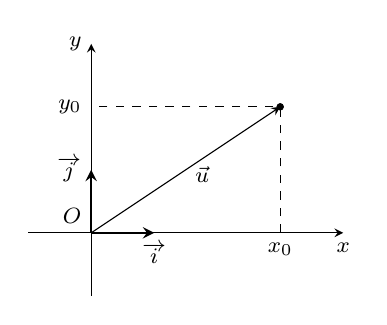
\begin{tikzpicture}[smooth,font=\footnotesize,scale=0.8,>=stealth]
	\draw[->] (-1,0)--(4,0) node [below]{$x$};
	\draw[->] (0,-1)--(0,3) node [left]{$y$};
	\draw[->,thick] (0,0)--(1,0) node [below]{$\overrightarrow{i}$};
	\draw[->,thick] (0,0)--(0,1) node [left]{$\overrightarrow{j}$};
	\draw (0,0) node[above left]{$O$};
	\draw[->] (0,0)--(3,2);
	\draw[dashed] (3,0)node [below]{$x_0$}--(3,2)--(0,2)node [left]{$y_0$} ;
	\draw [fill=black] (3,2) circle (.05);
	\node[below right] at (1.5,1.2){$\vec{u}$};
\end{tikzpicture}}


\subsubsection{Biểu thức tọa độ của các phép toán vectơ}
Cho hai vectơ $\overrightarrow{a}=\left( a_1;a_2 \right)$ và $\overrightarrow{b}=\left( b_1;b_2\right)$. Khi đó
\begin{tcolorbox}[colframe=cyan,colback=white,boxrule=0.2mm]
	\begin{listEX}[2]
		\item [\ding{172}] $\overrightarrow{a}+ \overrightarrow{b}=\left( a_1+ b_1;a_2+ b_2 \right)$ .
		\item [\ding{173}] $\overrightarrow{a}-\overrightarrow{b}=\left( a_1- b_1;a_2- b_2 \right)$ .
		\item [\ding{174}] $k\overrightarrow{a}=\left( ka_1;ka_2\right)$, với $k$ là một hằng số.
		\item [\ding{175}] $\overrightarrow{a}\cdot \overrightarrow{b}=a_1b_1+a_2b_2$
	\end{listEX}
\end{tcolorbox}
\subsubsection{Tọa độ điểm}

\immini{\begin{itemize}
		\item Xét điểm $M$ trên trục $(O,\overrightarrow{i}, \overrightarrow{j})$, ta luôn có $\overrightarrow{OM}=x_0\overrightarrow{i}+y_0\overrightarrow{j}$. Khi đó $(x_0,y_0)$ là tọa độ của $M$ trên hệ trục đã cho.
	\end{itemize}
		}{\vspace{-2cm}
	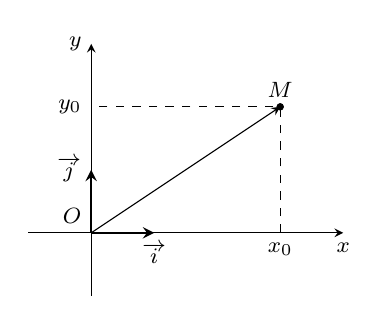
\begin{tikzpicture}[smooth,font=\footnotesize,scale=0.8,>=stealth]
		\draw[->] (-1,0)--(4,0) node [below]{$x$};
		\draw[->] (0,-1)--(0,3) node [left]{$y$};
		\draw[->,thick] (0,0)--(1,0) node [below]{$\overrightarrow{i}$};
		\draw[->,thick] (0,0)--(0,1) node [left]{$\overrightarrow{j}$};
		\draw (0,0) node[above left]{$O$};
		\draw[->] (0,0)--(3,2);
		\draw[dashed] (3,0)node [below]{$x_0$}--(3,2)node [above]{$M$}--(0,2)node [left]{$y_0$} ;
		\draw [fill=black] (3,2) circle (.05);
	\end{tikzpicture}}

\begin{itemize}
	\item Cho ba điểm $A\left( x_A;y_A \right)$, $B\left( x_B;y_B\right)$ và $C\left( x_C;y_C\right)$. Khi đó
	\begin{tcolorbox}[colframe=cyan,colback=white,boxrule=0.2mm]
		\begin{listEX}[1]
			\item [\ding{172}] $\overrightarrow{AB}=\left( x_B-x_A;y_B-y_A\right)$ 
			\item [\ding{173}] Khoảng cách giữa hai điểm $A$, $B$ là $AB=\sqrt{\left( x_B-x_A\right)^2+\left(y_B-y_A\right)^2}$.
			\item [\ding{174}] Trung điểm $I$ của $AB$:	$x_I=\dfrac{x_A+x_B}{2}$ và $y_I=\dfrac{y_A+y_B}{2}$
			\item [\ding{175}] $G$ là trọng tâm tam giác $ABC$: 
			$x_G=\dfrac{x_A+x_B+x_C}{3}$ và $y_G=\dfrac{y_A+y_B+y_C}{3}$.
			\item [\ding{176}] $ABC$ là ba đỉnh của tam giác $\Leftrightarrow $ $\overrightarrow{AB}$ không cùng phương với $\overrightarrow{AC}$
		\end{listEX}
	\end{tcolorbox}
\end{itemize}

\begin{dang}{Phân tích vectơ theo hai vectơ không cùng phương}
	Giả sử cần phân tích $\vec{u}=(u_1;u_2)$ theo hai vectơ không cùng phương $\vec{a}=(a_1;a_2)$ và $\vec{b}=(b_1;b_2)$. Ta thực hiện như sau:
	\begin{itemize}
		\item [$\bullet$] Giả sử $\vec{u} =m \cdot \vec{a} + n \cdot \vec{b}$ với $m,n \in \mathbb{R}$.
		\item [$\bullet$] Dùng điều kiện vectơ bằng nhau, ta được hệ
		$\heva{&u_1=m\cdot a_1 + n\cdot b_1\\&u_2=m\cdot a_2 + n\cdot b_2}.$
		\item [$\bullet$] Giải hệ trên tìm $m$ và $n$. Kết luận $\vec{u} =m \cdot \vec{a} + n \cdot \vec{b}$ với $m$, $n$ vừa tìm được.
	\end{itemize}	
\end{dang}

\begin{dang}{Ứng dụng biểu thức toạ độ của các phép toán vecttơ}
	Cho hai vectơ $\overrightarrow{a}=\left( a_1;a_2 \right)$ và $\overrightarrow{b}=\left( b_1;b_2\right)$.  
	\begin{itemize}
		\item [\ding{172}] $\overrightarrow{a}$ cùng phương $\overrightarrow{b} \Leftrightarrow a_1b_2-a_2b_1=0$.
		\item [\ding{173}] Chứng minh vuông góc: \fbox{$\overrightarrow{a}\perp \overrightarrow{b} \Leftrightarrow a_1b_1+a_2b_2=0$}.  
		\item [\ding{174}] Tính độ dài: $\boxed{|\overrightarrow{a}|=\sqrt{a_1^2+a_2^2}}$.
		\item [\ding{175}] Tính góc: $\boxed{\cos\left(\overrightarrow{a},\overrightarrow{b}\right)=\dfrac{\overrightarrow{a}\cdot \overrightarrow{b}}{|\overrightarrow{a}|\cdot\left|\overrightarrow{b}\right|}=\dfrac{a_1b_1+a_2b_2}{\sqrt{a_1^2+a_2^2}\cdot \sqrt{b_1^2+b_2^2}}}$ 
	\end{itemize}
\end{dang}


\begin{dang}{Xác định tọa độ các điểm đặc biệt trong tam giác}
	\begin{itemize}
		
		\item [\ding{172}] Xác định tọa độ trực tâm $H$ của tam giác $ABC$.
		\begin{gachsoc}
			\immini{\begin{itemize}
					\item [$\bullet$] Trực tâm $H$ là giao ba đường cao.
					\item [$\bullet$] Gọi $H(a;b)$ là trực tâm tam giác $ABC$.
					\item [$\bullet$] Giải hệ điều kiện $\heva{& \overrightarrow{AH} \cdot \overrightarrow{BC}=0\\& \overrightarrow{BH} \cdot \overrightarrow{AC}=0}$, tìm $a$, $b$.
				\end{itemize}
			}{
				\begin{tikzpicture}[scale=1, line join=round, line cap=round]
					\tkzDefPoints{0/0/B,3/0/C,1/2/A}
					\tkzDefPointBy[projection=onto C--B](A)\tkzGetPoint{K}
					\tkzDefPointBy[projection=onto A--B](C)\tkzGetPoint{E}
					\tkzDefPointBy[projection=onto C--A](B)\tkzGetPoint{F}
					\tkzInterLL(A,K)(C,E)\tkzGetPoint{H}	
					\pgfresetboundingbox
					\tkzDrawPolygon(A,B,C)
					\tkzDrawSegments(A,K C,E B,F)
					\tkzLabelPoints[below](B,C,K)
					\tkzLabelPoints[below right](H)
					\tkzLabelPoints[above](A)
					\tkzLabelPoints[right](F)
					\tkzLabelPoints[left](E)
			\end{tikzpicture}}
		\end{gachsoc}
		\item [\ding{173}] Xác định tọa độ hình chiếu vuông góc của $A$ lên $BC$
		\begin{gachsoc}
			\immini{\begin{itemize}
					\item [$\bullet$] Gọi $K(a;b)$ là hình chiếu vuông góc của $A$ lên $BC$.
					\item [$\bullet$] Giải hệ điều kiện $\heva{& \overrightarrow{AK} \cdot \overrightarrow{BC}=0\\& \overrightarrow{BK} \text{ cùng phương } \overrightarrow{BC}}$, tìm $a$, $b$.
				\end{itemize}
			}{
				\begin{tikzpicture}[scale=1, line join=round, line cap=round]
					\tkzDefPoints{0/0/B,3/0/C,1/2/A}
					\tkzDefPointBy[projection=onto C--B](A)\tkzGetPoint{K}
					\tkzDefPointBy[projection=onto A--B](C)\tkzGetPoint{E}
					\tkzDefPointBy[projection=onto C--A](B)\tkzGetPoint{F}
					\pgfresetboundingbox
					\tkzDrawPolygon(A,B,C)
					\tkzDrawSegments(A,K C,E B,F)
					\tkzLabelPoints[below](B,C,K)
					\tkzLabelPoints[above](A)
					\tkzLabelPoints[right](F)
					\tkzLabelPoints[left](E)
			\end{tikzpicture}}
		\end{gachsoc}
		\item [\ding{174}] Xác định tọa độ tâm đường tròn ngoại tiếp tam giác $ABC$.
		\begin{gachsoc}
			\immini{\begin{itemize}
					\item [$\bullet$] Tâm đường tròn ngoại tiếp là giao của ba đường trung trực.
					\item [$\bullet$] Gọi $I(a;b)$ là tâm đường tròn ngoại tiếp tam giác $ABC$.
					\item [$\bullet$] Giải hệ điều kiện $\heva{& IA =IB\\& IA=IC}$, tìm $a$, $b$.
				\end{itemize}
			}{
				\begin{tikzpicture}[scale=0.9, line join=round, line cap=round]
					\tkzDefPoints{0/0/B,3/0/C,1/2/A}
					\tkzCircumCenter(A,B,C)\tkzGetPoint{I}
					\tkzDrawCircle[circum](A,B,C)
					\tkzDrawSegments(I,A I,B I,C)
					\tkzDrawPolygon(A,B,C)
					\tkzLabelPoints[below,font=\footnotesize](I)
					\tkzLabelPoints[above,font=\footnotesize](A)
					\tkzLabelPoints[below left,font=\footnotesize](B)
					\tkzLabelPoints[below right,font=\footnotesize](C)
			\end{tikzpicture}}
		\end{gachsoc}
		\item [\ding{175}] Xác định tọa độ tâm đường tròn nội tiếp tam giác $ABC$.
		\begin{gachsoc}
			\immini{\begin{itemize}
					\item [$\bullet$] Tính độ dài $AB$, $AC$.
					\item [$\bullet$] Áp dụng tính chất phân giác trong tam giác $ABC$, ta có 
					$$\dfrac{DB}{DC}=\dfrac{AB}{AC}=k_1 \Rightarrow \overrightarrow{DB}=k_1\overrightarrow{DC} $$ Từ đây, tìm tọa độ điểm $D$.
					\item [$\bullet$] Áp dụng tính chất phân giác trong tam giác $BAD$, ta có 
					$$\dfrac{JA}{JD}=\dfrac{BA}{BD}= k_2\Rightarrow \overrightarrow{JA}=-k_2\overrightarrow{JD}$$ Từ đây, tìm tọa độ điểm $J$.
				\end{itemize}
			}{
				\begin{tikzpicture}[scale=1, line join=round, line cap=round]
					\tkzDefPoints{0/0/B,3/0/C,1/2/A}
					\tkzInCenter(A,B,C)\tkzGetPoint{J}
					\tkzInterLL(A,J)(C,B)\tkzGetPoint{D}
					\tkzDrawSegments(A,D B,J)
					\tkzDrawPolygon(A,B,C)
					\tkzDrawPoints[size=3,fill=black](A,B,C,D,J)
					\tkzLabelPoints[below,font=\footnotesize](D)
					\tkzLabelPoints[above,font=\footnotesize](A)
					\tkzLabelPoints[below left,font=\footnotesize](B)
					\tkzLabelPoints[below right,font=\footnotesize](C,J)
					%\tkzDrawCircle[in](A,B,C)					
			\end{tikzpicture}}
		\end{gachsoc}
		\begin{luuy}
			Đặt $a=BC$, $b=AC$ và $c=AB$. Ta có công thức tính trực tiếp $$x_J=\dfrac{a\cdot x_A+b \cdot x_B+c \cdot x_C}{a+b+c};\,\,y_J=\dfrac{a\cdot y_A+b \cdot y_B+c \cdot y_C}{a+b+c}$$
		\end{luuy}
	\end{itemize}
\end{dang}


